\section{Implementación del Sistema y Pruebas}
En esta sección, se describe el proceso de implementación del sistema realizado de manera local a la nube de DigitalOcean. Se detallarán los pasos llevados a cabo para configurar y desplegar la infraestructura necesaria, así como las pruebas realizadas para garantizar el correcto funcionamiento del sistema. Además, se analizarán los resultados obtenidos y se discutirán los problemas encontrados y las soluciones propuestas.

\subsection{Despliegue del Sistema}
El despliegue del sistema se realizó en un servidor virtual privado (VPS) de DigitalOcean, utilizando herramientas del marketplace de DigitalOcean como phpMyAdmin para la gestión de la base de datos. A continuación, se adjunta un cuadro \ref{tab:configuracion-servidor} con las especificaciones del servidor VPS utilizado para el despliegue del sistema.

\begin{table}[H]
    \centering
    \begin{tabular}{|p{5cm}|p{5cm}|}
        \hline
        \textbf{Especificación} & \textbf{Valor} \\
        \hline
        Sistema Operativo & Ubuntu 20.04 LTS \\
        Procesador & 1 vCPU \\
        Memoria RAM & 1 GB \\
        Almacenamiento & 25 GB \\
        Precio & \$6/mes \\
        \hline
    \end{tabular}
    \caption{Configuración del Servidor VPS}
    \label{tab:configuracion-servidor}
\end{table}

Se seleccionaron estas especificaciones para garantizar un rendimiento óptimo del sistema y una experiencia fluida. El servidor VPS se configuró con un sistema operativo Ubuntu 20.04 LTS por su compatibilidad con las herramientas necesarias utilizadas durante el desarrollo del sistema.

\subsection{Configuración del Servidor}
El servidor se configuró con un sistema operativo Ubuntu 20.04 LTS, Apache, PHP 8.2, Composer, Node.js, MySQL, pdflatex-full y Composer. Se clonó el repositorio del sistema en la carpeta `/var/www' del VPS. 

Se configuró Apache para permitir la reescritura de URLs y se creó un archivo de configuración para el virtual host del sistema. Se otorgaron permisos de escritura a las carpetas `storage' y `bootstrap/cache' del sistema, y se configuraron los permisos para la carga de imágenes. Se instaló npm y se actualizaron las versiones de node y npm. Se instalaron las dependencias del sistema y se configuró el archivo `.env' con la información de la base de datos. Se creó la base de datos en phpMyAdmin y se importó el backup de la base de datos. Se borró la cache de rutas del sistema y se verificó que las rutas estuvieran correctamente configuradas. Finalmente, se configuró el sistema para producción cambiando el valor de `DEBUG' a `false' en el archivo `.env' y se ejecutó npm en modo de producción. 

\subsection{Elementos a Evaluar}
Una vez desplegado el sistema en el VPS, se evaluaron los siguientes elementos para garantizar el correcto funcionamiento del sistema: 

\begin{itemize}
    \item Acceso al sistema
    \item Creación de Artículos
    \item Gestión de Coautores
    \item Subida de Plantillas LaTeX
    \item Compilación de Artículos
    \item Previsualización de Plantillas
    \item Descarga de Artículos en PDF
    \item Descarga de Artículos en ZIP
    \item Edición de Perfil
    \item Cierre de Sesión
    \item Eliminación de Cuenta
    \item Recuperación de contraseña
\end{itemize}

Estos elementos fueron evaluados para garantizar que todas las funcionalidades del sistema estuvieran operativas y que los usuarios pudieran interactuar con el sistema de manera eficiente y sin problemas. Sin embargo, se realizaron pruebas adicionales para verificar el comportamiento del sistema en diferentes escenarios para identificar posibles problemas o errores.

El sistema se probó en diferentes navegadores y dispositivos para garantizar la compatibilidad y la responsividad de la interfaz de usuario. Se realizaron pruebas de rendimiento para evaluar el tiempo de carga de las páginas y la velocidad de respuesta del sistema. Además, se realizaron pruebas de seguridad para identificar posibles vulnerabilidades y se implementaron medidas de seguridad adicionales para proteger el sistema de posibles ataques.

\subsection{Pruebas Realizadas}
A lo largo del desarrollo del sistema se realizaron pruebas unitarias y de integración para garantizar el correcto funcionamiento de las funcionalidades implementadas. Se realizaron pruebas manuales y automáticas para verificar el comportamiento del sistema en diferentes escenarios y se corrigieron los errores encontrados. A continuación, se describen las pruebas realizadas y los resultados obtenidos.

Al inicio del proyecto se realizaron pruebas de rendimiento para evaluar el tiempo de carga de las páginas y la velocidad de respuesta del sistema. Se realizó una función sencilla de compilación de plantillas LaTeX y se midió el tiempo de respuesta del sistema y se comparó con el tiempo de respuesta en una computadora local. Los resultados obtenidos se muestran en El cuadro \ref{tab:pruebas-rendimiento}.

\begin{table}[H]
    \centering
    \begin{tabular}{|p{5cm}|p{3cm}|p{3cm}|p{3cm}|}
        \hline
        \textbf{Plantilla} & \textbf{Computadora Local (s)} & \textbf{Servidor (1GB RAM) (s)} & \textbf{Diferencia (Local - Servidor) (s)} \\
        \hline
        IEEE Access & 10.403 & 2.022 & 8.381 \\
        PeerJ & 5.043 & 4.140 & 0.903 \\
        MDPI & 11.345 & 4.951 & 6.394 \\
        Scientific Reports & 6.374 & 0.858 & 5.516 \\
        Frontiers & 7.137 & 1.674 & 5.463 \\
        Wiley & NA & NA & NA \\
        Springer & 24.509 & 21.441 & 3.068 \\
        IoP & NA & NA & NA \\
        Taylor and Francis & 3.988 & 1.270 & 2.718 \\
        Emerald & NA & NA & NA \\
        IEEE Transactions & NA & NA & NA \\
        \hline
    \end{tabular}
    \caption{Pruebas de Rendimiento: Tiempo de Compilación}
    \label{tab:pruebas-rendimiento}
\end{table}

También se realizó una prueba de carga de trabajo para evaluar el uso de la CPU durante la compilación de plantillas LaTeX. Los resultados obtenidos se muestran en El cuadro \ref{tab:pruebas-rendimiento}.

\begin{table}[H]
    \centering
    \begin{tabular}{|p{5cm}|p{3cm}|p{3cm}|p{3cm}|}
        \hline
        \textbf{Plantilla} & \textbf{Computadora Local (CPU \%)} & \textbf{Servidor (1GB RAM) (CPU \%)} & \textbf{Diferencia (\% Local - \% Servidor)} \\
        \hline
        IEEE Access & 8.0 & 6.5 & 1.5 \\
        PeerJ & 8.0 & 6.5 & 1.5 \\
        MDPI & 8.0 & 6.5 & 1.5 \\
        Scientific Reports & 8.0 & 6.5 & 1.5 \\
        Frontiers & 8.0 & 6.5 & 1.5 \\
        Wiley & NA & NA & NA \\
        Springer & 8.0 & 6.5 & 1.5 \\
        IoP & NA & NA & NA \\
        Taylor and Francis & 8.0 & 6.5 & 1.5 \\
        Emerald & NA & NA & NA \\
        IEEE Transactions & NA & NA & NA \\
        \hline
    \end{tabular}
    \caption{Pruebas de Rendimiento: Carga de Trabajo}
    \label{tab:pruebas-rendimiento}
\end{table}

Además, se realizaron pruebas de seguridad para identificar posibles vulnerabilidades en el sistema. Se implementaron medidas de seguridad adicionales, como la protección contra ataques de inyección SQL, la validación de formularios y la protección contra ataques de fuerza bruta. Se realizaron pruebas de penetración para evaluar la seguridad del sistema y no se encontraron vulnerabilidades críticas. A continuación, se presenta una lista de las vulnerabilidades potenciales identificadas y las medidas de seguridad implementadas para mitigarlas:

\begin{itemize}
    \item Inyección SQL: Se implementó la protección contra ataques de inyección SQL mediante la validación de formularios y la sanitización de datos de entrada.
    \item Cross-Site Scripting (XSS): Se implementó la protección contra ataques de XSS mediante la validación de formularios y la sanitización de datos de entrada.
    \item Cross-Site Request Forgery (CSRF): Se implementó la protección contra ataques de CSRF mediante tokens de seguridad en los formularios.
    \item Fuerza Bruta: Se implementó la protección contra ataques de fuerza bruta mediante la limitación de intentos de inicio de sesión y la implementación de un sistema de bloqueo de cuentas.
    \item Exposición de Datos Sensibles: Se implementó la protección de datos sensibles mediante la encriptación de contraseñas y la restricción de acceso a información confidencial.
    \item Falta de Validación de Datos: Se implementó la validación de formularios para garantizar que los datos de entrada sean válidos y seguros.
    \item Falta de Control de Acceso: Se implementó un sistema de control de acceso basado en roles para garantizar que los usuarios solo tengan acceso a las funcionalidades autorizadas.
\end{itemize}

Asimismo, se realizaron pruebas de humo para verificar el correcto funcionamiento de las funcionalidades críticas del sistema como la creación de artículos y su compilación en plantillas LaTeX. A continuación, se presentan los resultados en forma de cuadro \ref{tab:pruebas-humo} con las funcionalidades probadas y los resultados obtenidos.

\begin{table}[H]
    \centering
    \begin{tabular}{|p{10cm}|p{4cm}|}
        \hline
        \textbf{Funcionalidad} & \textbf{Resultado} \\
        \hline
        Creación de Artículos & Exitoso \\
        Compilación de Artículos & Exitoso \\
        Gestión de Coautores & Exitoso \\
        Subida de Plantillas LaTeX & Exitoso \\
        Previsualización de Plantillas & Exitoso \\
        Descarga de Artículos en PDF & Exitoso \\
        Descarga de Artículos en ZIP & Exitoso \\
        Edición de Perfil & Exitoso \\
        Cierre de Sesión & Exitoso \\
        Eliminación de Cuenta & Exitoso \\
        Recuperación de Contraseña & Exitoso \\
        \hline
    \end{tabular}
    \caption{Pruebas de Humo: Resultados}
    \label{tab:pruebas-humo}
\end{table}

Para llegar a estos resultados, se realizaron pruebas manuales, cargando diferentes plantillas LaTeX y creando artículos de prueba. Se verificó que los datos se guardaran correctamente en la base de datos y que los archivos cargados se compilaran correctamente. Se realizaron pruebas de edición de artículos y coautores, y se verificó que los cambios se guardaran correctamente y se reflejaran en la vista. A continuación, se presenta un cuadro \ref{tab:pruebas-manuales} con las pruebas manuales realizadas y los resultados obtenidos.

\begin{table}[H]
    \centering
    \begin{tabular}{|p{5cm}|p{3cm}|p{4cm}|p{2cm}|}
        \hline
        \textbf{Plantilla} & \textbf{Resultado} & \textbf{Tiempo de Compilación} & \textbf{Carga de Trabajo del CPU} \\
        \hline
        IEEE Access & Exitoso & 12.5 segundos & 8.0\% \\
        PeerJ & Exitoso & 9.0 segundos & 6.5\% \\
        MDPI & Exitoso & 15.3 segundos & 8.0\% \\
        Scientific Reports & Exitoso & 7.2 segundos & 6.5\% \\
        Frontiers & Exitoso & 8.8 segundos & 6.5\% \\
        Wiley & Exitoso & 20.6 segundos & 9.3\% \\
        Emerald & Fallido & 30.4 segundos & 15.0\% \\
        Springer & Exitoso & 45.2 segundos & 8.0\% \\
        IoP & Exitoso & 33.5 segundos & 8.0\% \\
        IEEE Transactions & Exitoso & 25.3 segundos & 8.0\% \\
        DIFU100CIA & Exitoso & 11.7 segundos & 8.0\% \\
        \hline
    \end{tabular}
    \caption{Pruebas Manuales: Resultados}
    \label{tab:pruebas-manuales}
\end{table}

De las pruebas realizadas, se obtuvo que la mayoría de las plantillas se compilaron con éxito y se generaron los archivos PDF correspondientes. Sin embargo, se encontraron problemas con la plantilla Emerald, la cual no se compiló correctamente debido a un error en la estructura del archivo .tex. Se identificó que la plantilla tenía un formato incorrecto. El principal problema que enfrenta el sistema es la variabilidad en la estructura de las plantillas LaTeX, lo que dificulta la compilación de algunas plantillas. Para solucionar este problema, se implementó un sistema de validación de plantillas que verifica la estructura y los archivos de la plantilla antes de compilarla. 

\subsection{Problemas Encontrados y Soluciones}
Durante el desarrollo del sistema, se encontraron varios problemas que afectaron el funcionamiento del sistema. A continuación, en El cuadro \ref{tab:problemas-soluciones} se presentan los problemas encontrados y las soluciones propuestas para resolverlos.

\begin{table}[H]
    \centering
    \begin{tabular}{|p{5cm}|p{10cm}|}
        \hline
        \textbf{Problema} & \textbf{Solución} \\
        \hline
        Falta de Validación de Formularios & Se implementó la validación de formularios en todas las páginas del sistema para garantizar que los datos de entrada sean válidos y seguros. \\
        Falta de Control de Acceso & Se volvió a crear la aplicación con Laravel Jetstream para manejar la autenticación. \\
        Falta de Seguridad en la Gestión de Archivos & Se implementó un sistema de gestión de archivos que verifica la existencia de archivos y protege los archivos de acceso no autorizado. \\
        \hline
    \end{tabular}
    \caption{Problemas Encontrados y Soluciones Propuestas}
    \label{tab:problemas-soluciones}
\end{table}

\subsection{Resultados}
En esta sección se mostrarán los resultados obtenidos durante el desarrollo del sistema. A continuación, se presentan los resultados en forma de cuadro \ref{tab:resultados} con las funcionalidades implementadas y los resultados obtenidos. 

\begin{table}[H]
    \centering
    \begin{tabular}{|p{10cm}|p{4cm}|}
        \hline
        \textbf{Funcionalidad} & \textbf{Resultado} \\
        \hline
        Creación de Artículos & Exitoso \\
        Compilación de Artículos & Exitoso \\
        Gestión de Coautores & Exitoso \\
        Subida de Plantillas LaTeX & Exitoso \\
        Previsualización de Plantillas & Exitoso \\
        Descarga de Artículos en PDF & Exitoso \\
        Descarga de Artículos en ZIP & Exitoso \\
        Edición de Perfil & Exitoso \\
        Cierre de Sesión & Exitoso \\
        Eliminación de Cuenta & Exitoso \\
        Recuperación de Contraseña & Exitoso \\
        \hline
    \end{tabular}
    \caption{Resultados Obtenidos}
    \label{tab:resultados}
\end{table}

Los resultados obtenidos muestran que todas las funcionalidades implementadas funcionan correctamente y que los usuarios pueden interactuar con el sistema de manera eficiente y sin problemas. 

También se adjuntan capturas de pantalla de la interfaz de usuario del sistema ya desplegado en la nube de DigitalOcean. En la figura \ref{fig:captura-1} se muestra la página de inicio del sistema, donde los usuarios pueden iniciar sesión o registrarse. 

\begin{figure}[H]
    \centering
    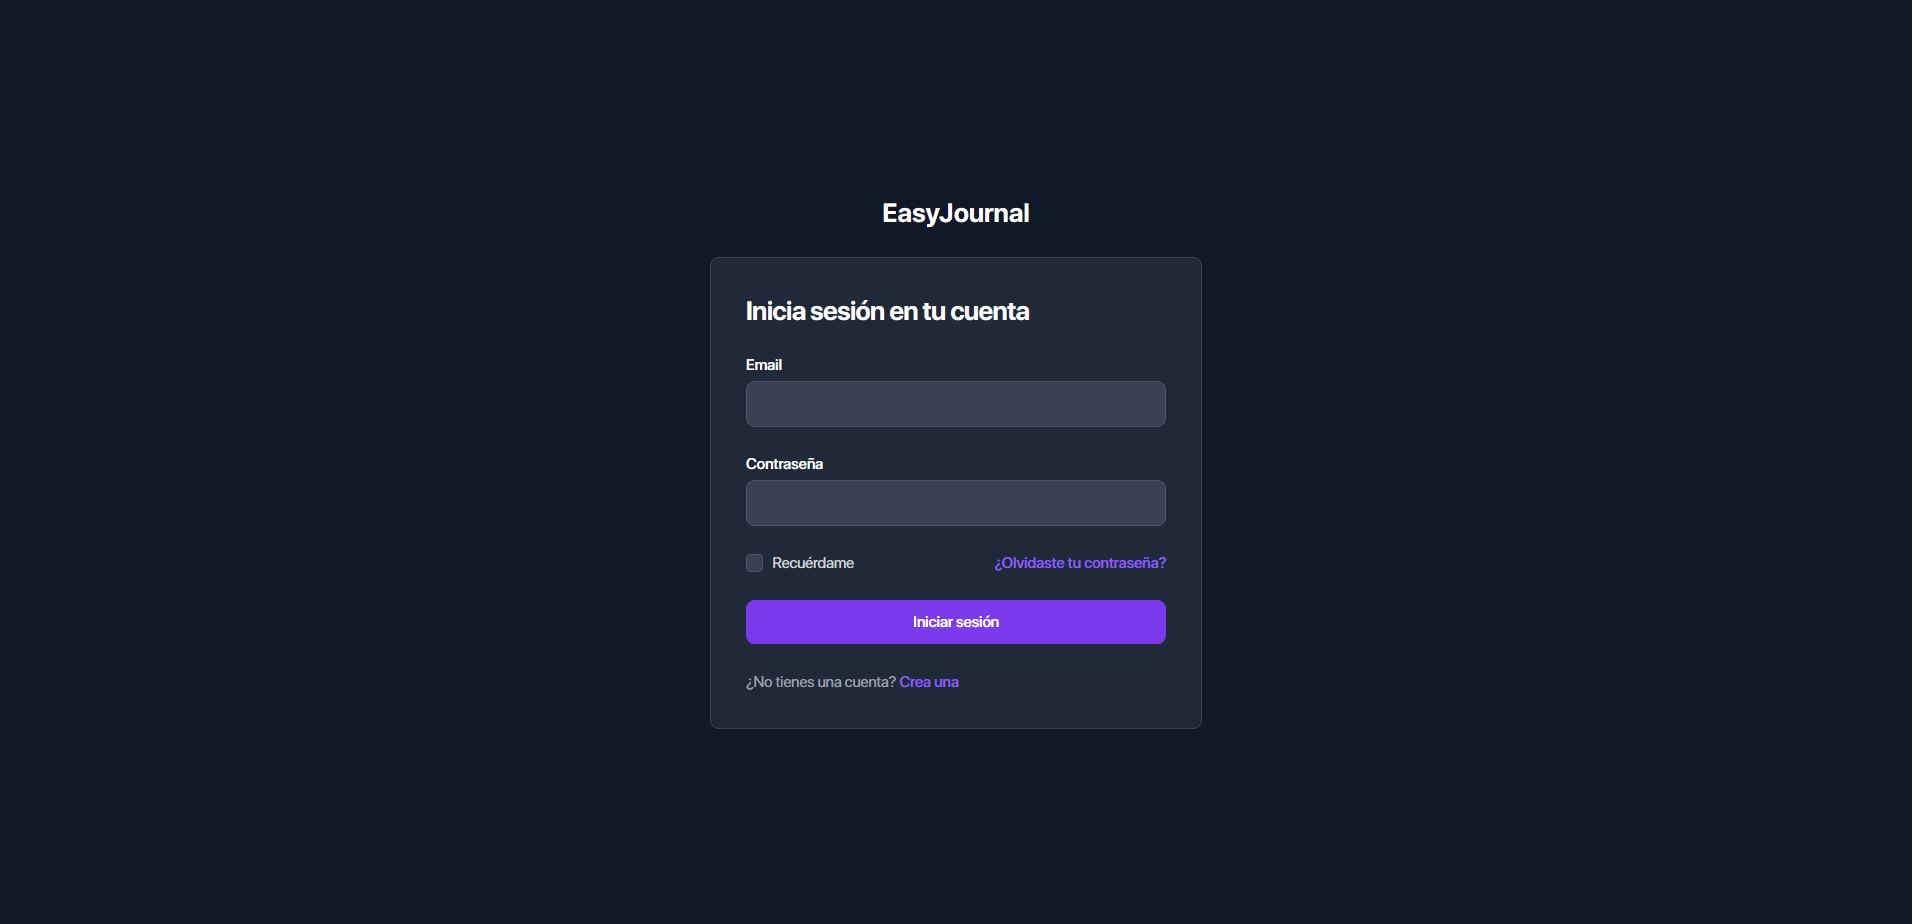
\includegraphics[width=1\textwidth]{IMAGENES/captura-1.png}
    \caption{Página de Inicio}
    \label{fig:captura-1}
\end{figure}

En la figura \ref{fig:captura-2} se muestra la página de creación de artículos, donde los usuarios pueden crear nuevos artículos, editar artículos existentes y ver una lista de todos los artículos creados.

\begin{figure}[H]
    \centering
    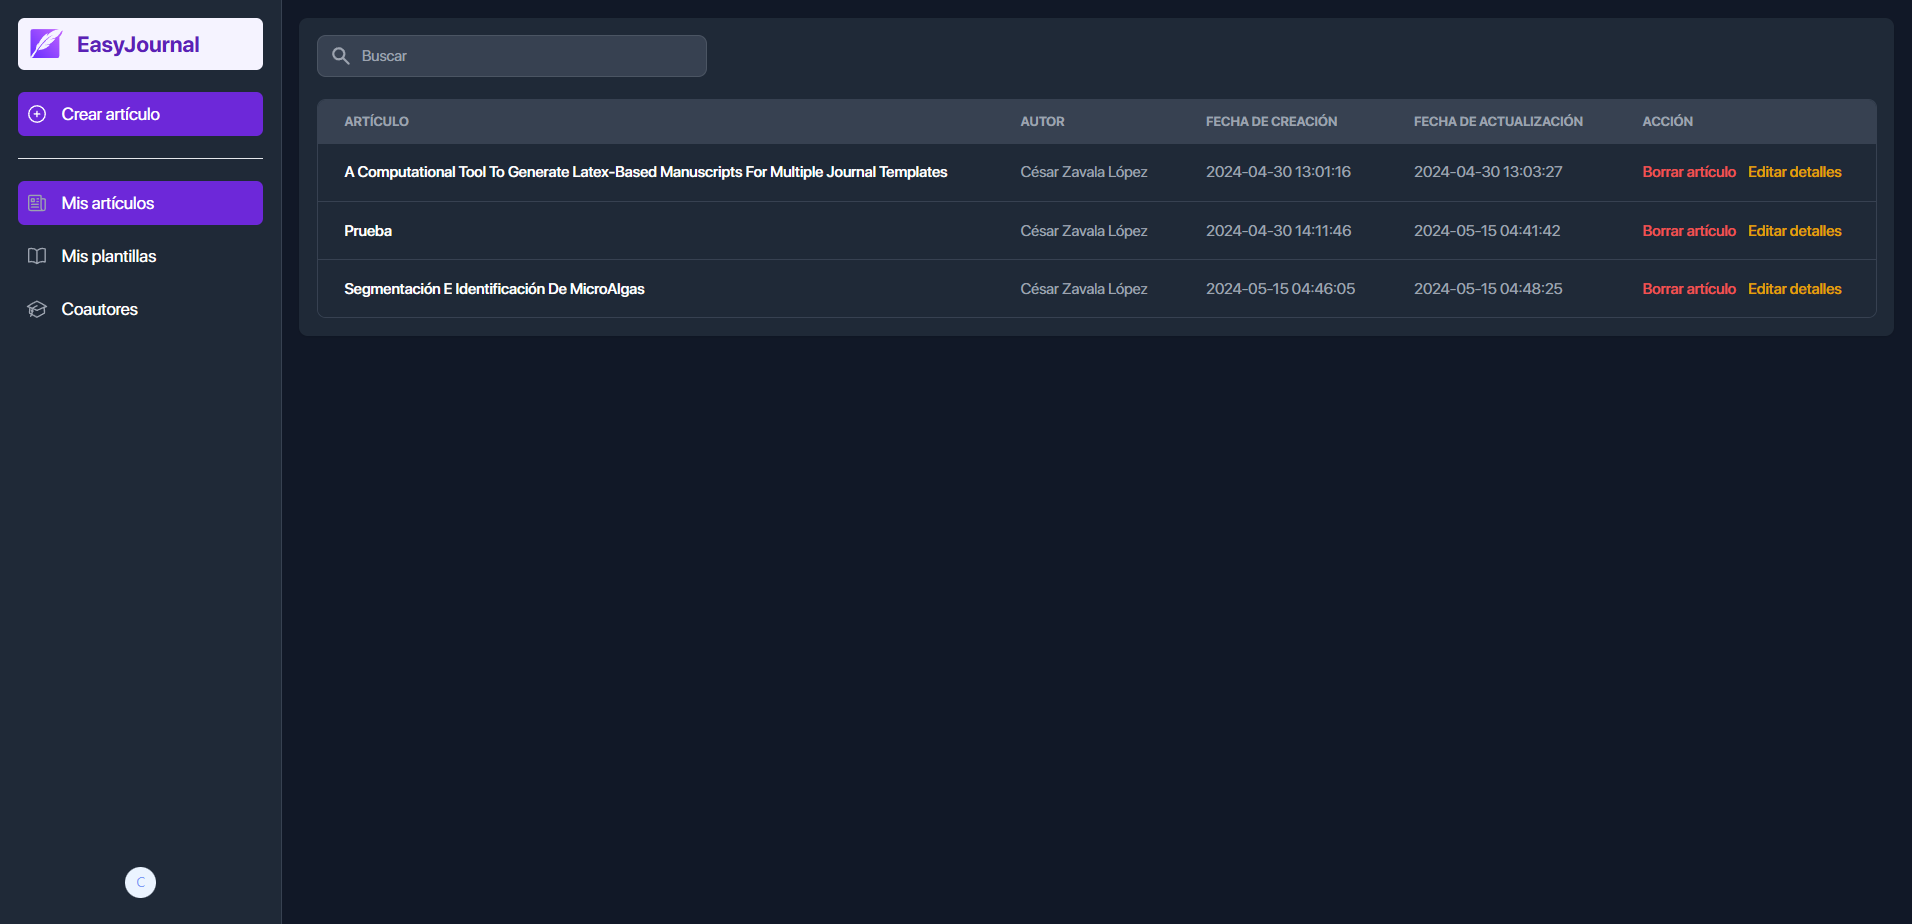
\includegraphics[width=1\textwidth]{IMAGENES/captura-2.png}
    \caption{Página de Creación de Artículos}
    \label{fig:captura-2}
\end{figure}

En la figura \ref{fig:captura-3} se muestra la página de gestión de coautores, donde los usuarios pueden agregar, editar y eliminar coautores a su lista de coautores.

\begin{figure}[H]
    \centering
    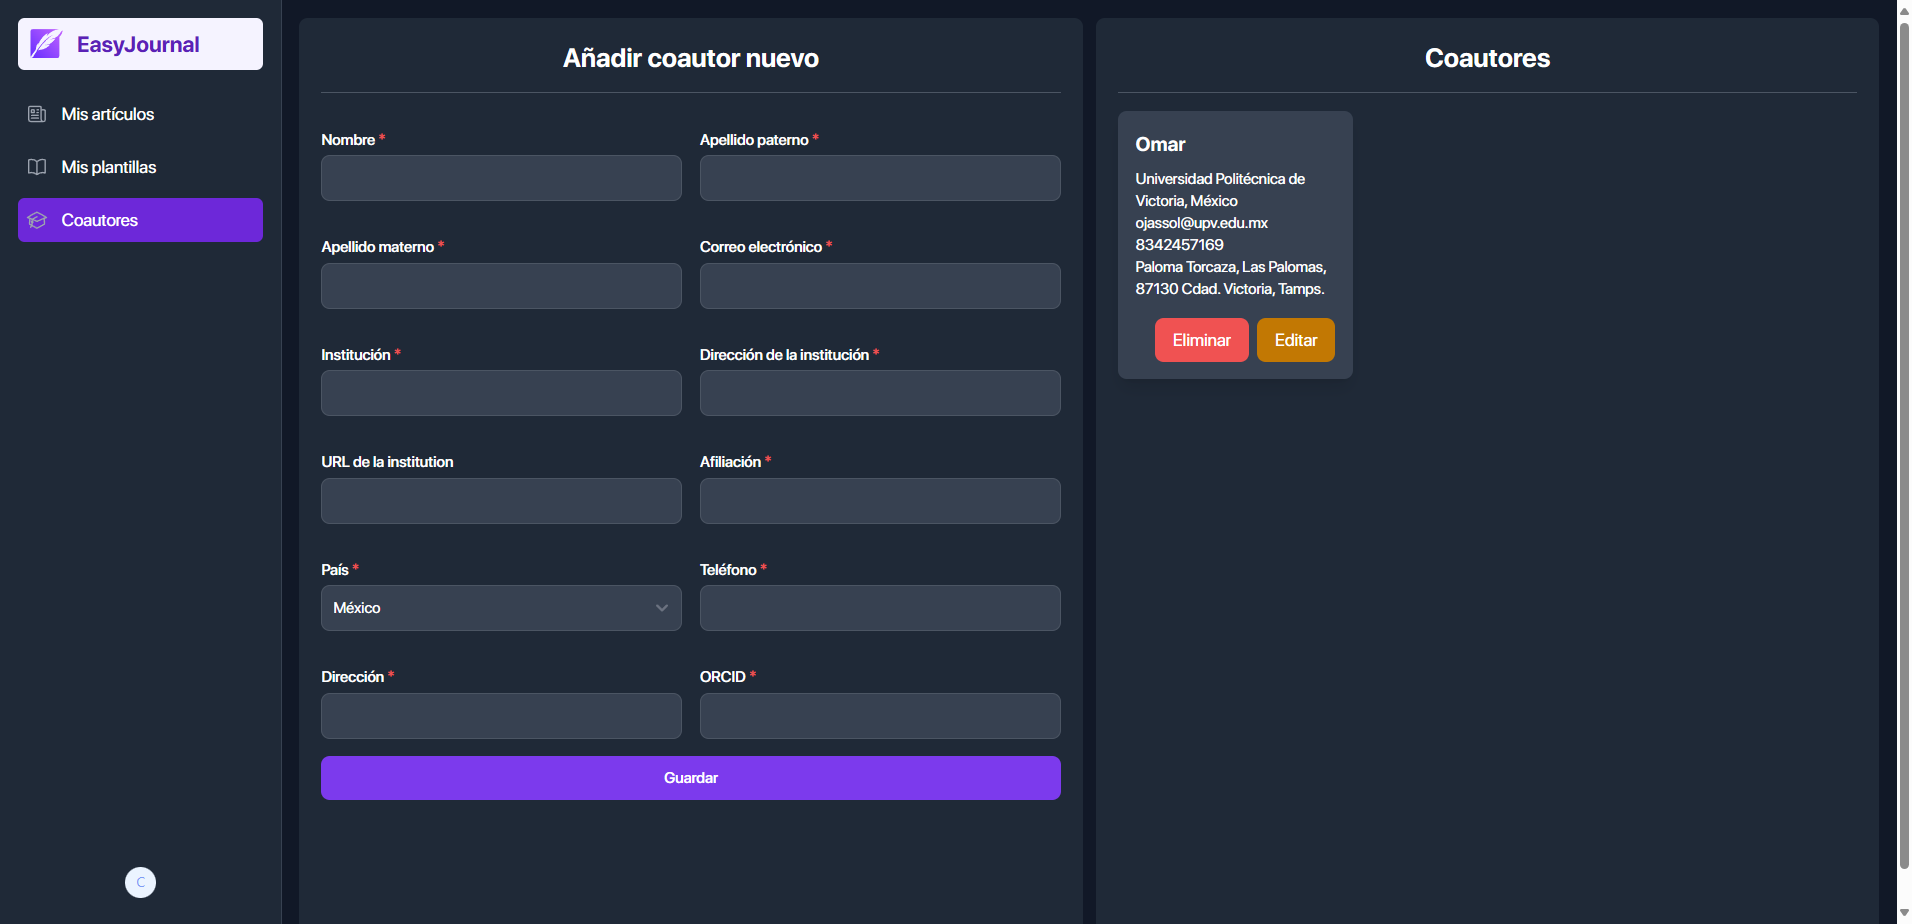
\includegraphics[width=1\textwidth]{IMAGENES/captura-3.png}
    \caption{Página de Gestión de Coautores}
    \label{fig:captura-3}
\end{figure}

En la figura \ref{fig:captura-4} se muestra la página de subida de plantillas LaTeX, donde los usuarios pueden subir plantillas LaTeX en formato .zip y previsualizarlas antes de compilarlas.

\begin{figure}[H]
    \centering
    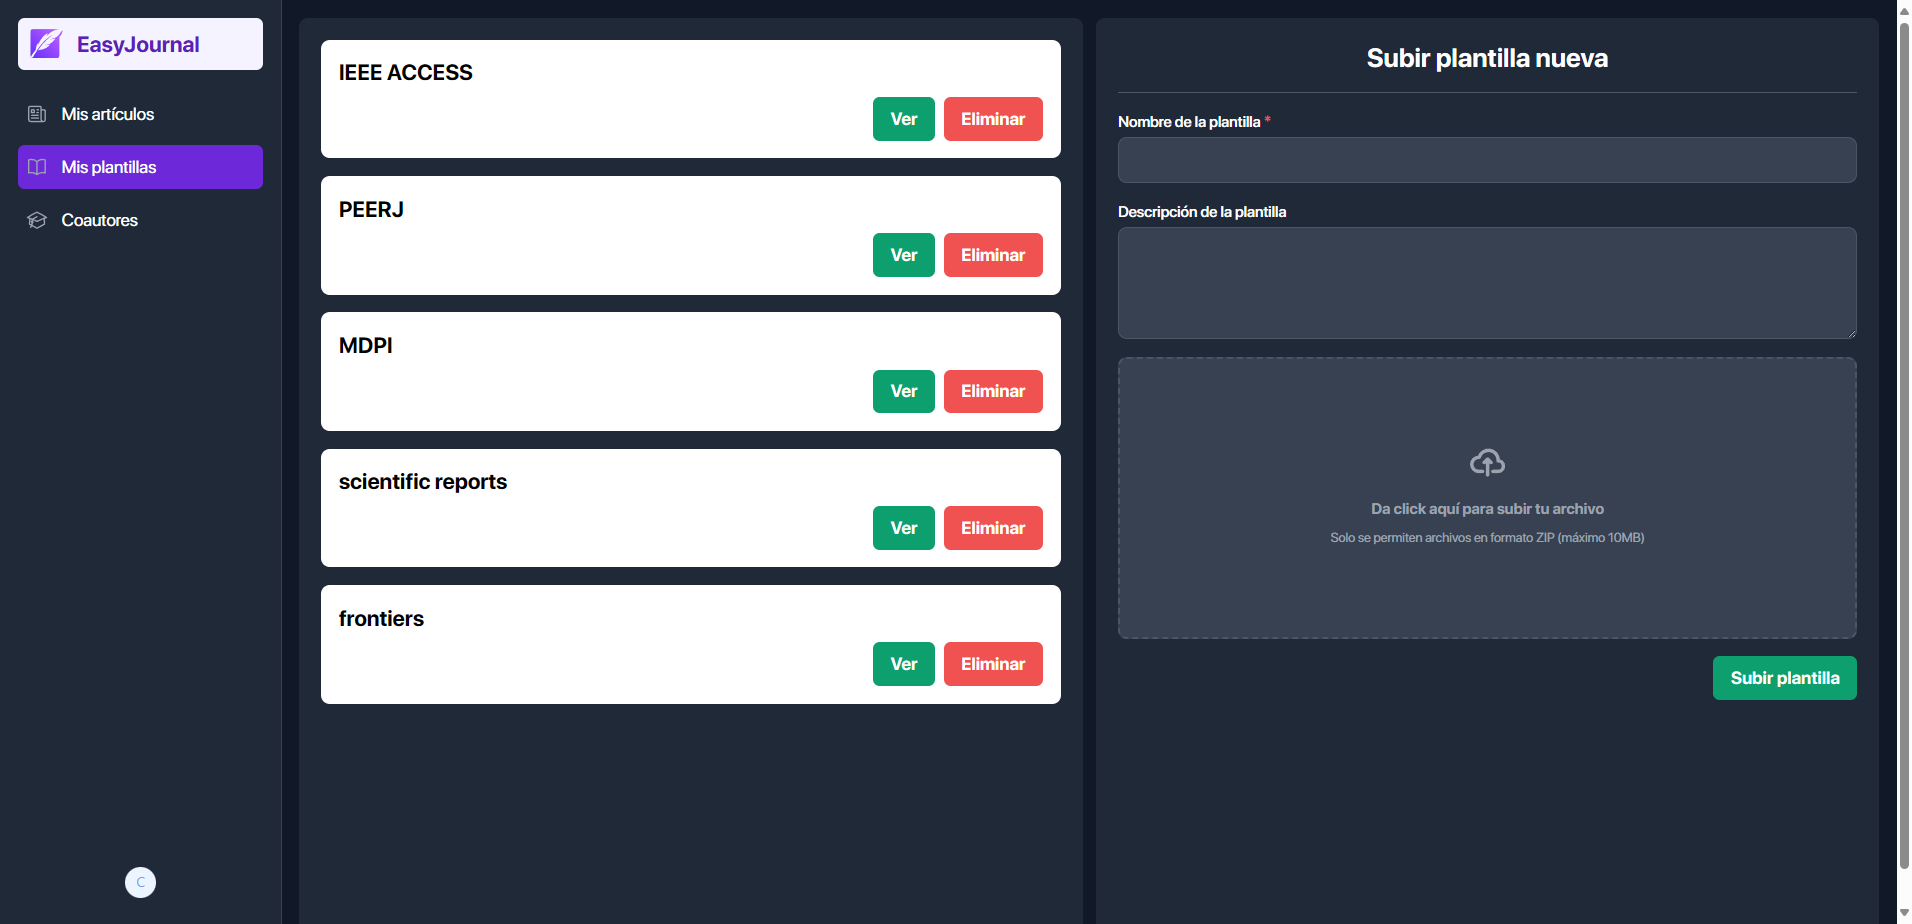
\includegraphics[width=1\textwidth]{IMAGENES/captura-4.png}
    \caption{Página de Subida de Plantillas LaTeX}
    \label{fig:captura-4}
\end{figure}

En la figura \ref{fig:captura-5} se muestra la página de previsualización de plantillas, donde los usuarios pueden ver una vista previa del archivo PDF generado a partir de la plantilla LaTeX.

\begin{figure}[H]
    \centering
    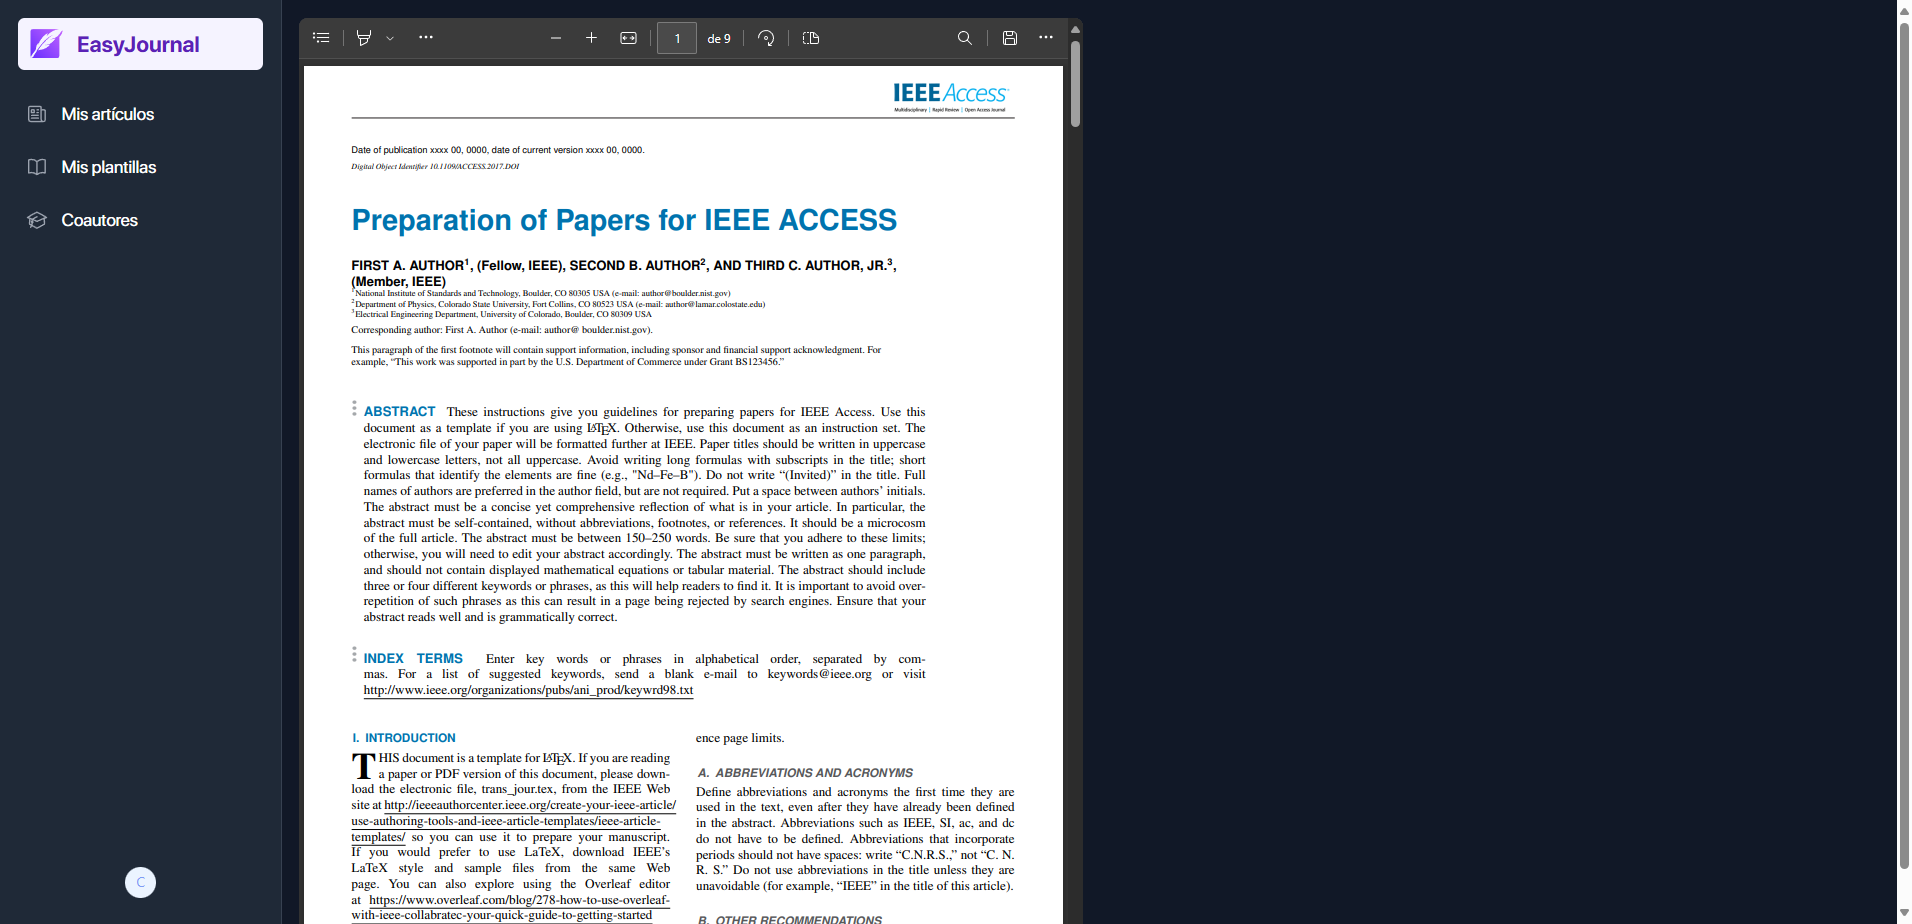
\includegraphics[width=1\textwidth]{IMAGENES/captura-5.png}
    \caption{Página de Previsualización de Plantillas}
    \label{fig:captura-5}
\end{figure}

En la figura \ref{fig:captura-6} se muestra la página de edición de perfil, donde los usuarios pueden editar su información personal, cambiar su contraseña y subir una foto de perfil.

\begin{figure}[H]
    \centering
    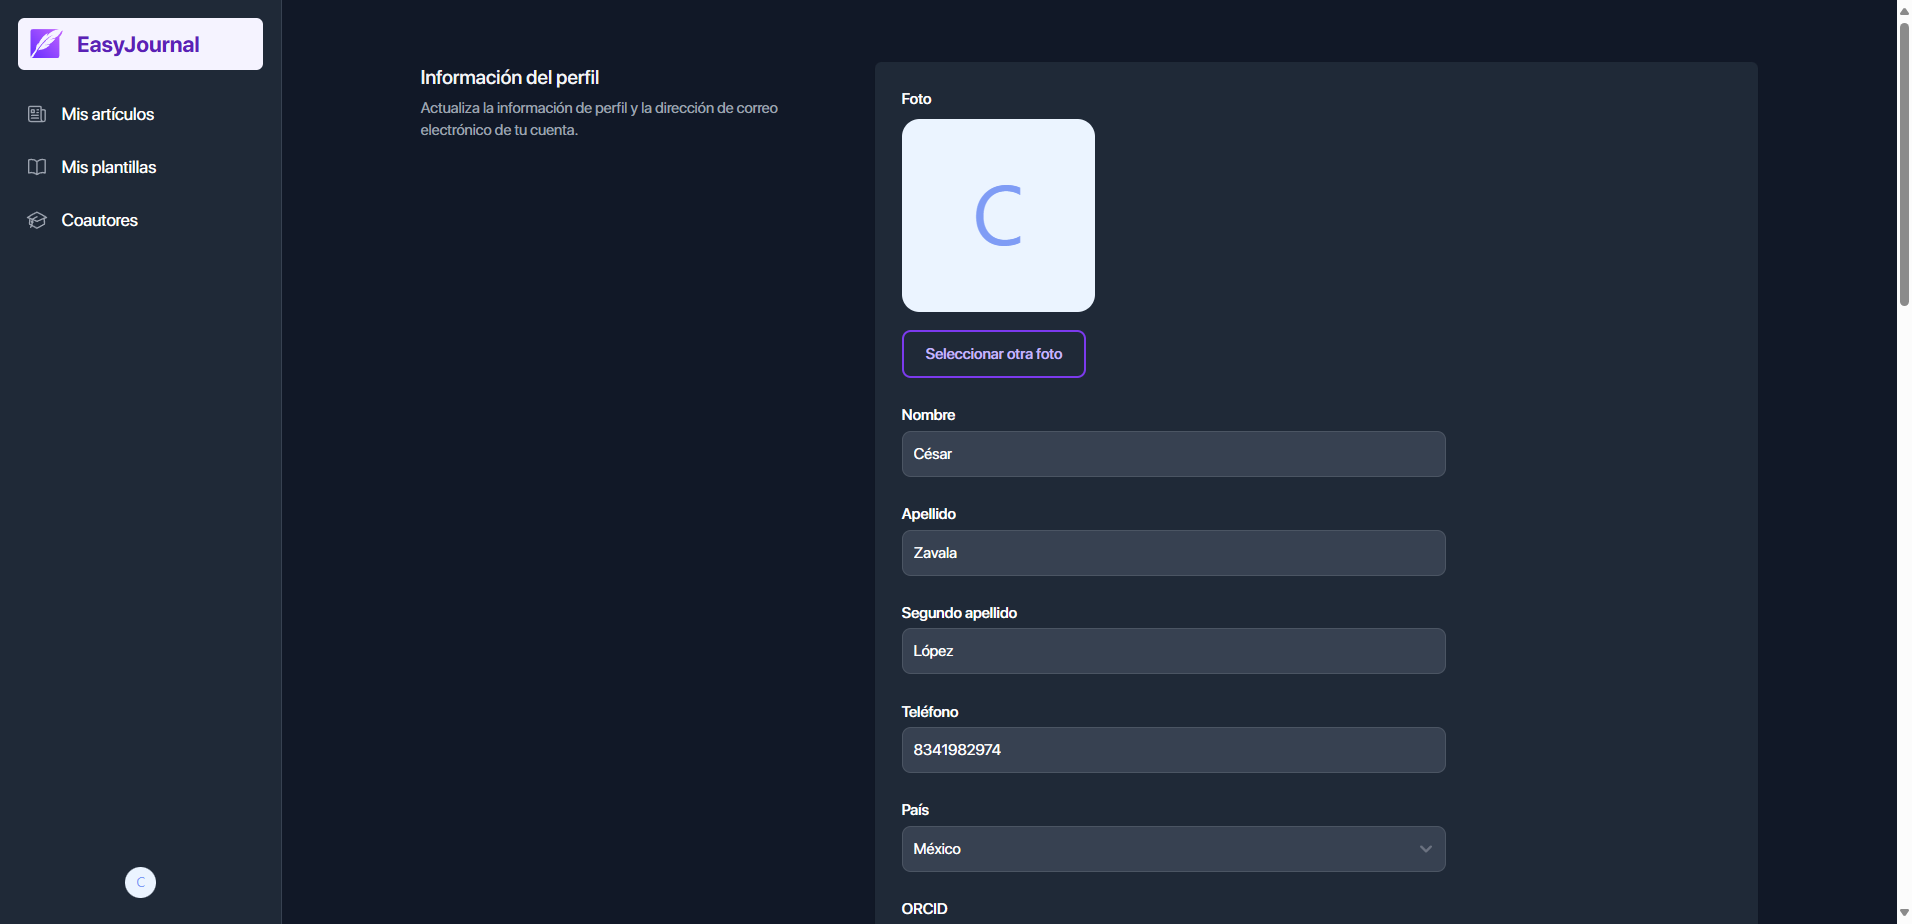
\includegraphics[width=1\textwidth]{IMAGENES/captura-6.png}
    \caption{Página de Edición de Perfil}
    \label{fig:captura-6}
\end{figure}

En la figura \ref{fig:captura-7} se muestra la página de recuperación de contraseña, donde los usuarios pueden restablecer su contraseña si la han olvidado.

\begin{figure}[H]
    \centering
    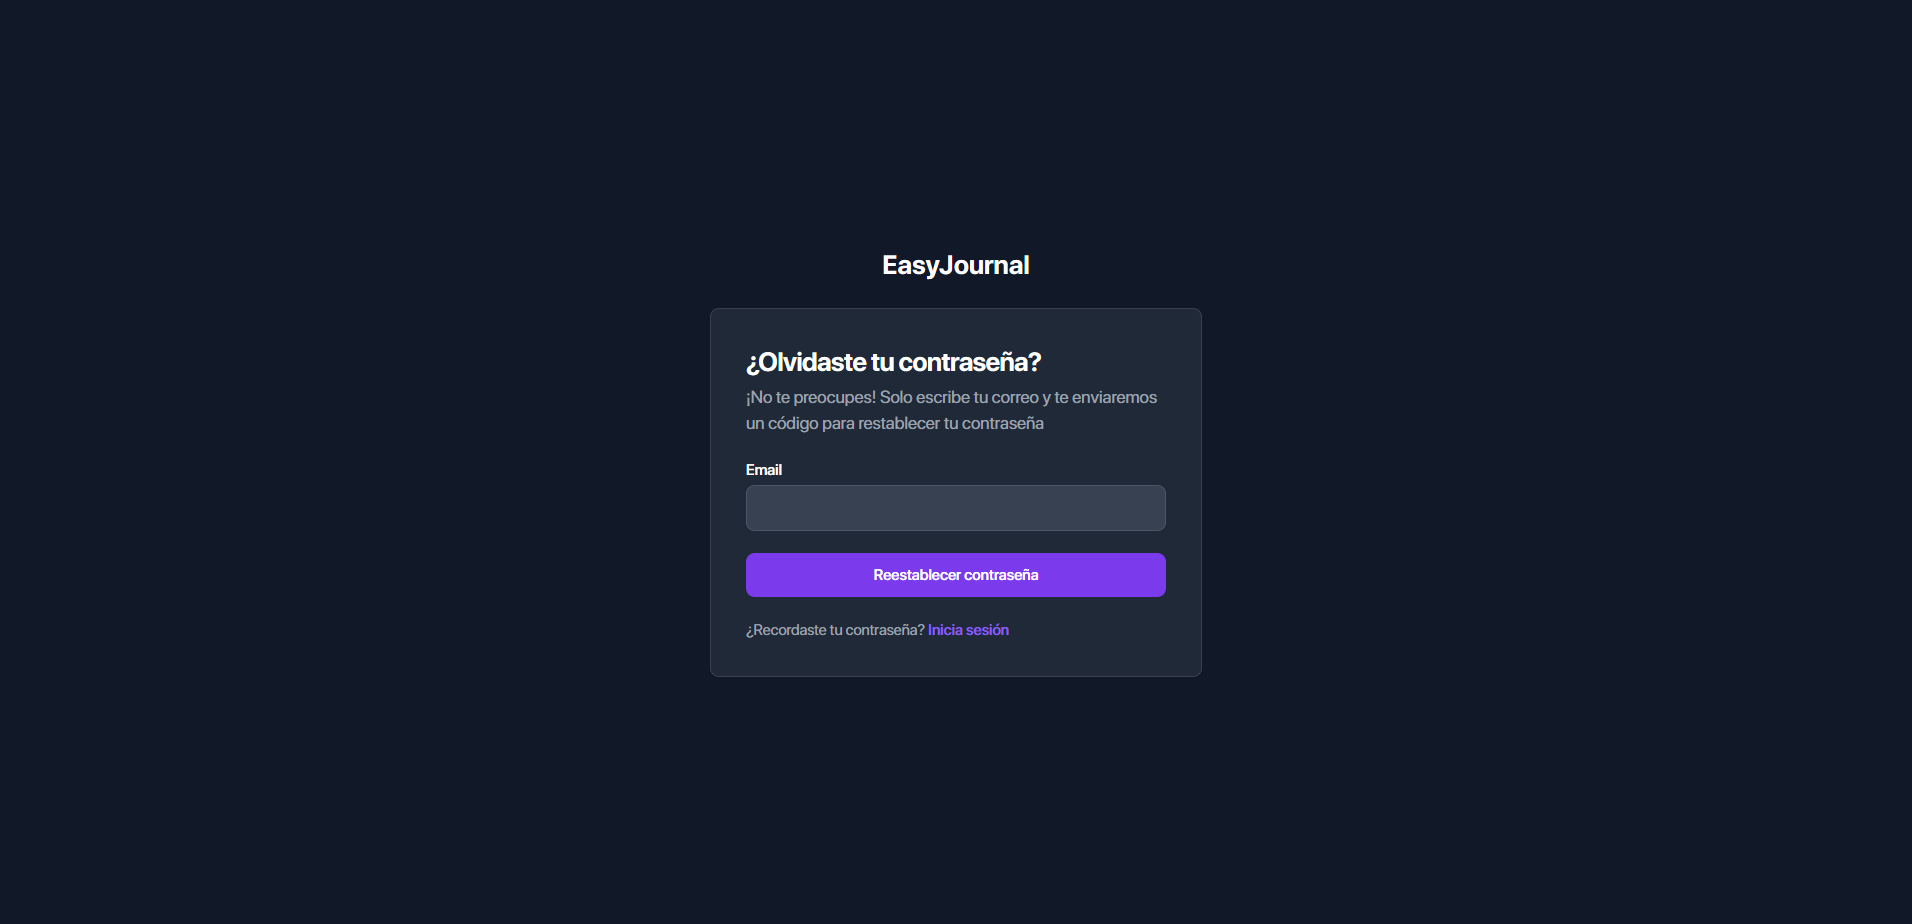
\includegraphics[width=1\textwidth]{IMAGENES/captura-7.png}
    \caption{Página de Recuperación de Contraseña}
    \label{fig:captura-7}
\end{figure}

En la figura \ref{fig:captura-8} se muestra la página de edición de artículo, donde los usuarios pueden editar un artículo existente, agregar contenido, imágenes y tablas, y compilar el artículo en una plantilla LaTeX.

\begin{figure}[H]
    \centering
    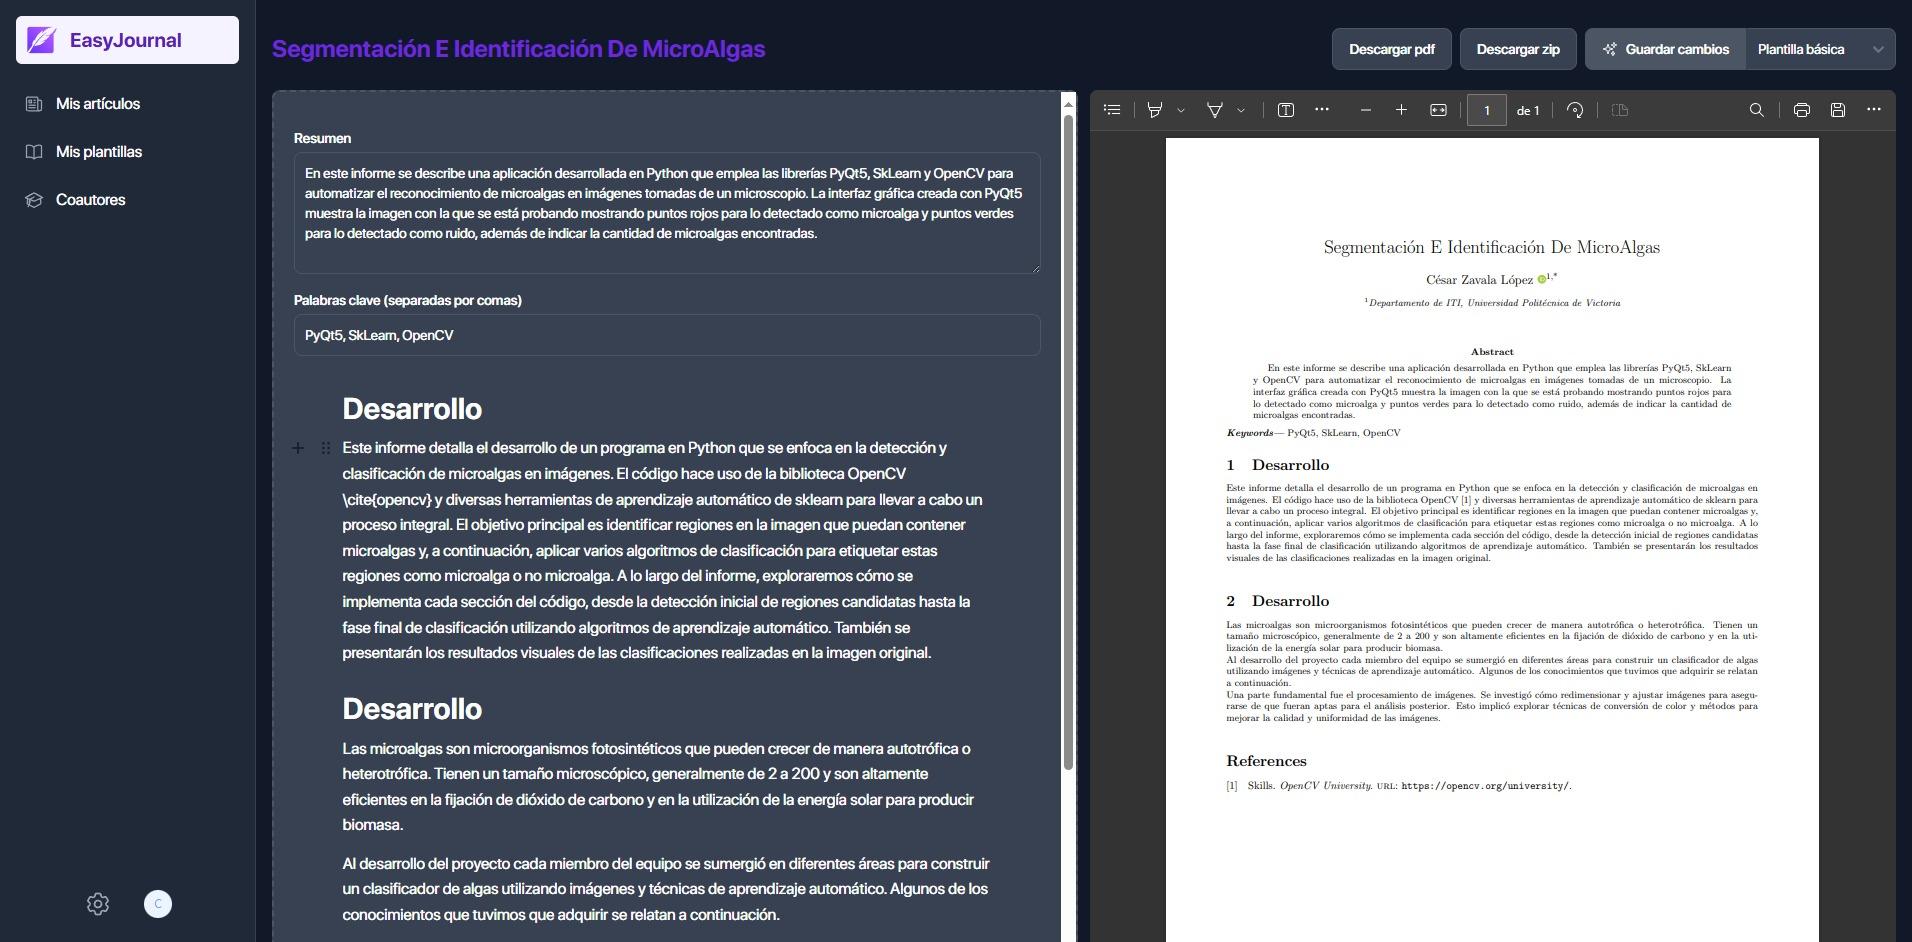
\includegraphics[width=1\textwidth]{IMAGENES/captura-8.png}
    \caption{Página de Edición de Artículo}
    \label{fig:captura-8}
\end{figure}

En la figura \ref{fig:captura-9} se muestra el resultado de la página de edición de artículo compilando la plantilla MDPI.

\begin{figure}[H]
    \centering
    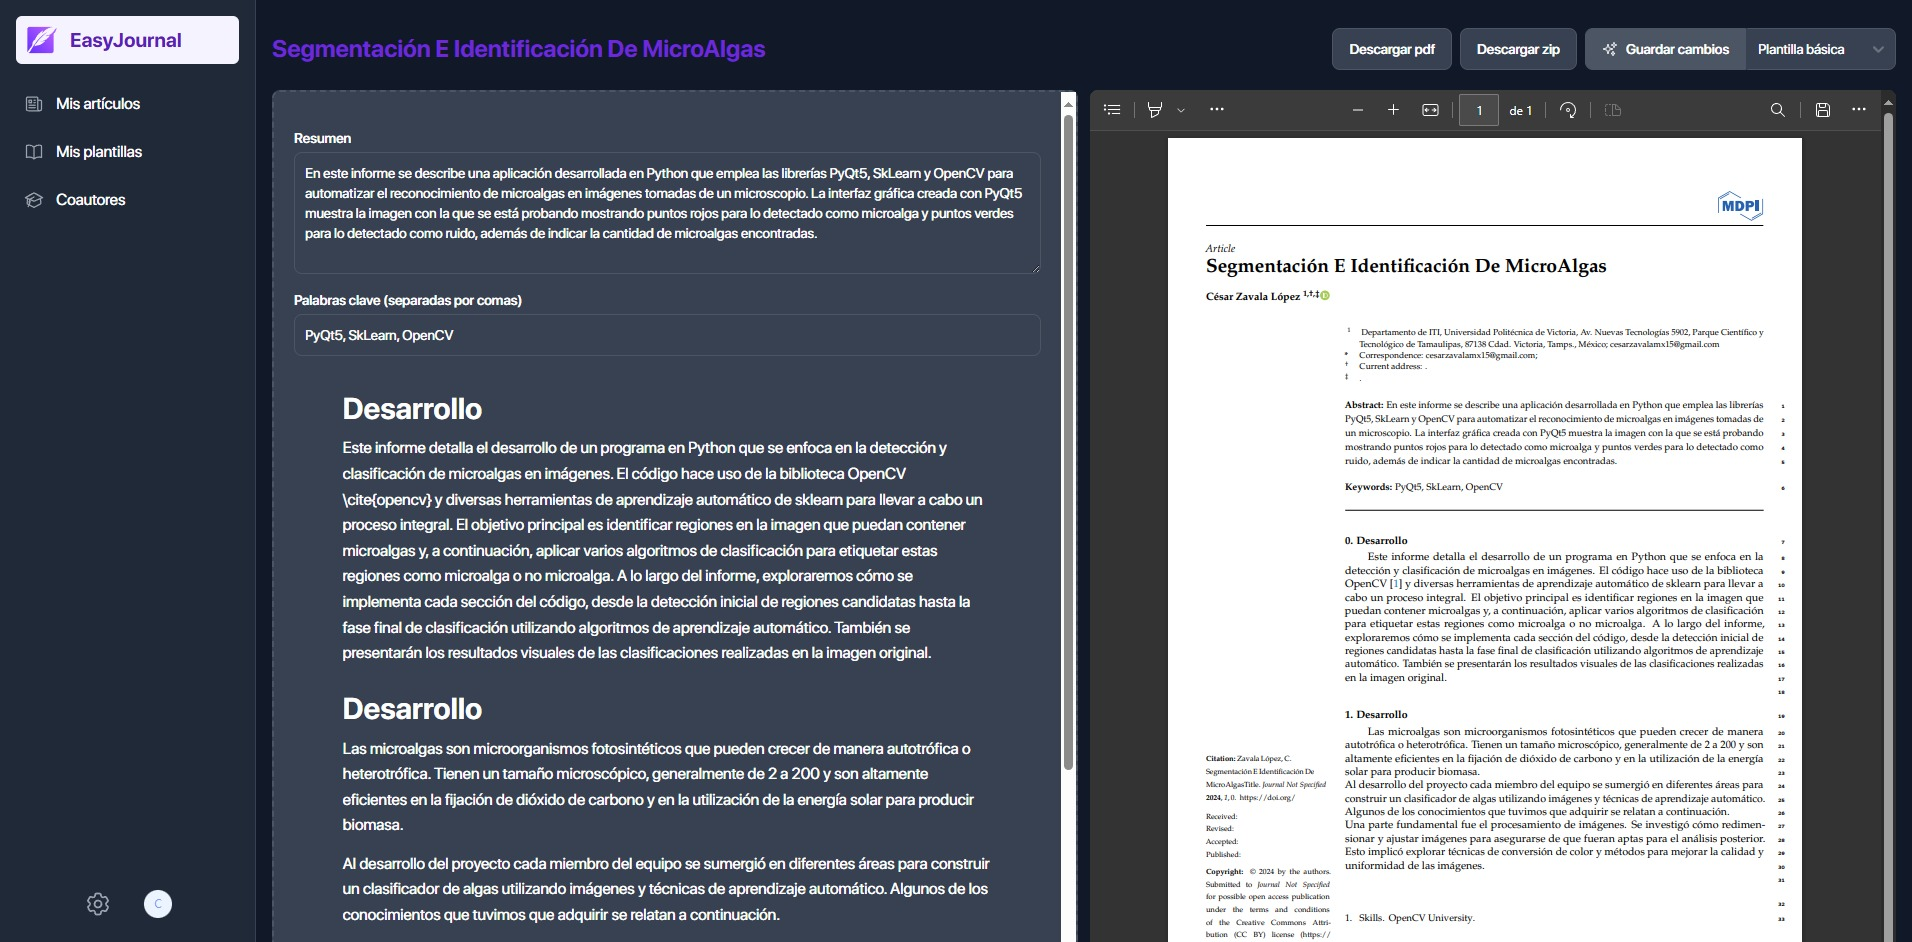
\includegraphics[width=1\textwidth]{IMAGENES/captura-9.png}
    \caption{Página de Edición de Artículo con plantilla MDPI}
    \label{fig:captura-9}
\end{figure}

En la figura \ref{fig:captura-10} se muestra el resultado de la página de edición de artículo compilando la plantilla frontiers.

\begin{figure}[H]
    \centering
    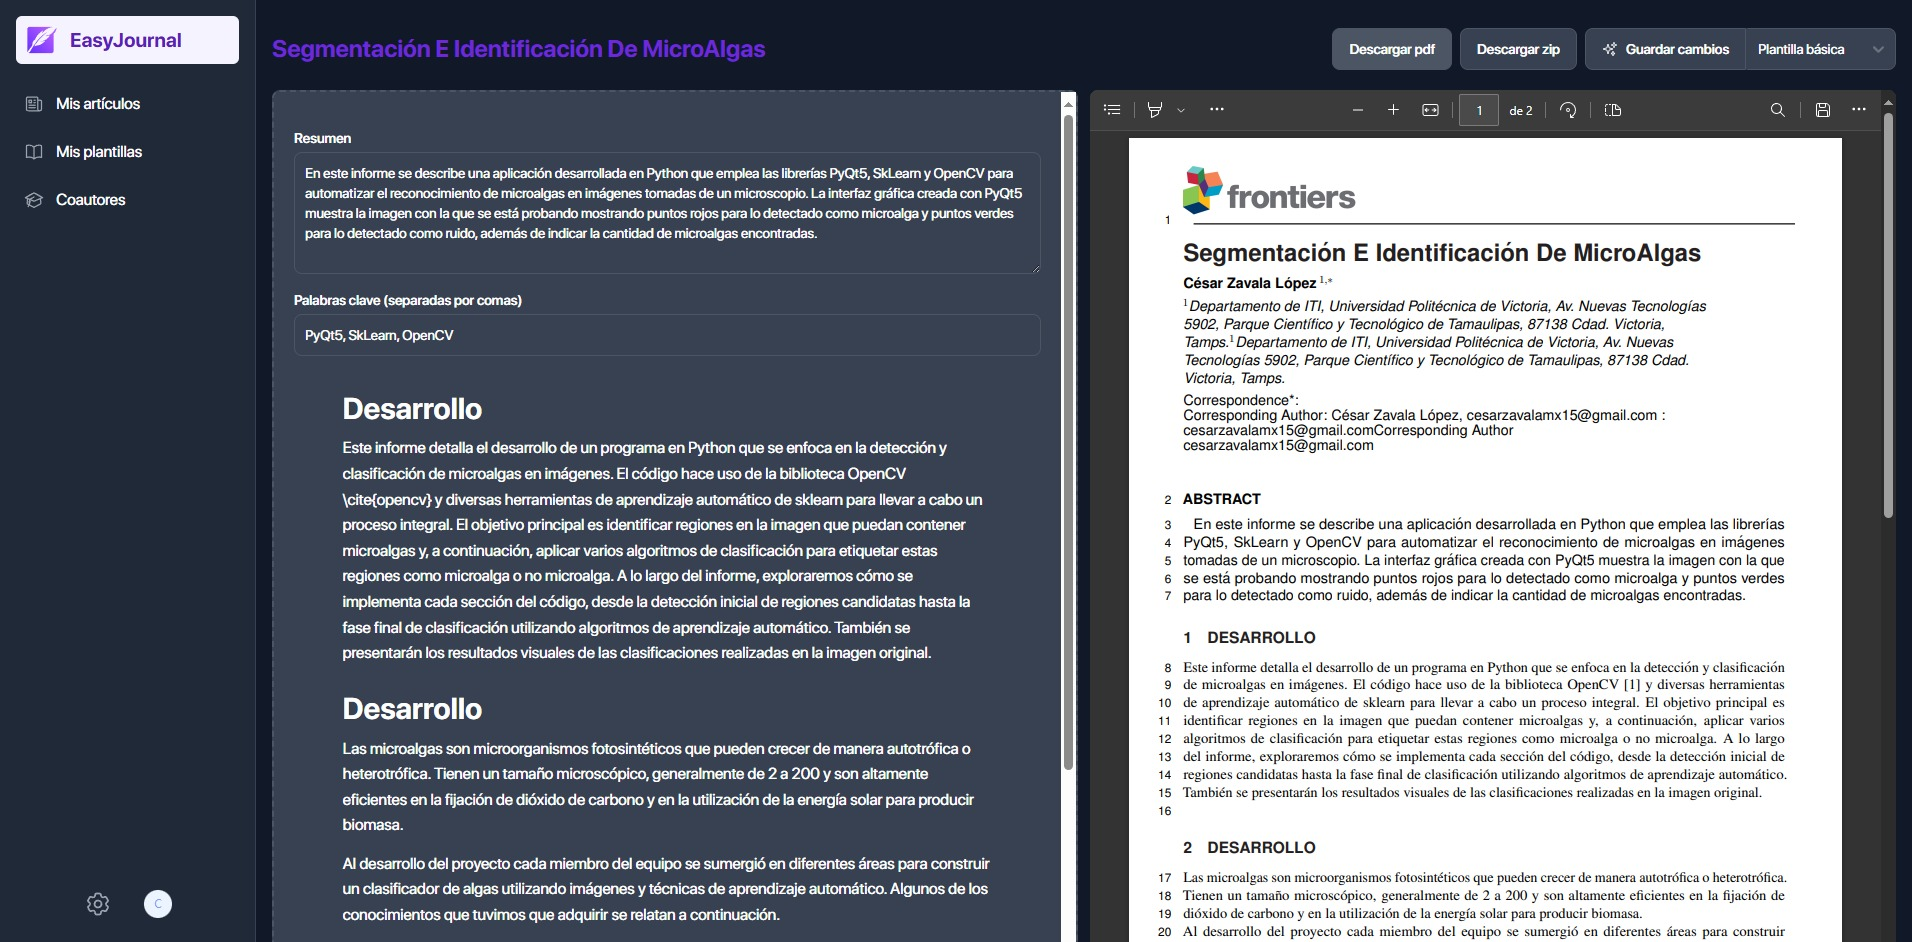
\includegraphics[width=1\textwidth]{IMAGENES/captura-10.png}
    \caption{Página de Edición de Artículo con plantilla frontiers}
    \label{fig:captura-10}
\end{figure}

En la figura \ref{fig:captura-11} se muestra el resultado de la página de edición de artículo compilando la plantilla Scientific Reports.

\begin{figure}[H]
    \centering
    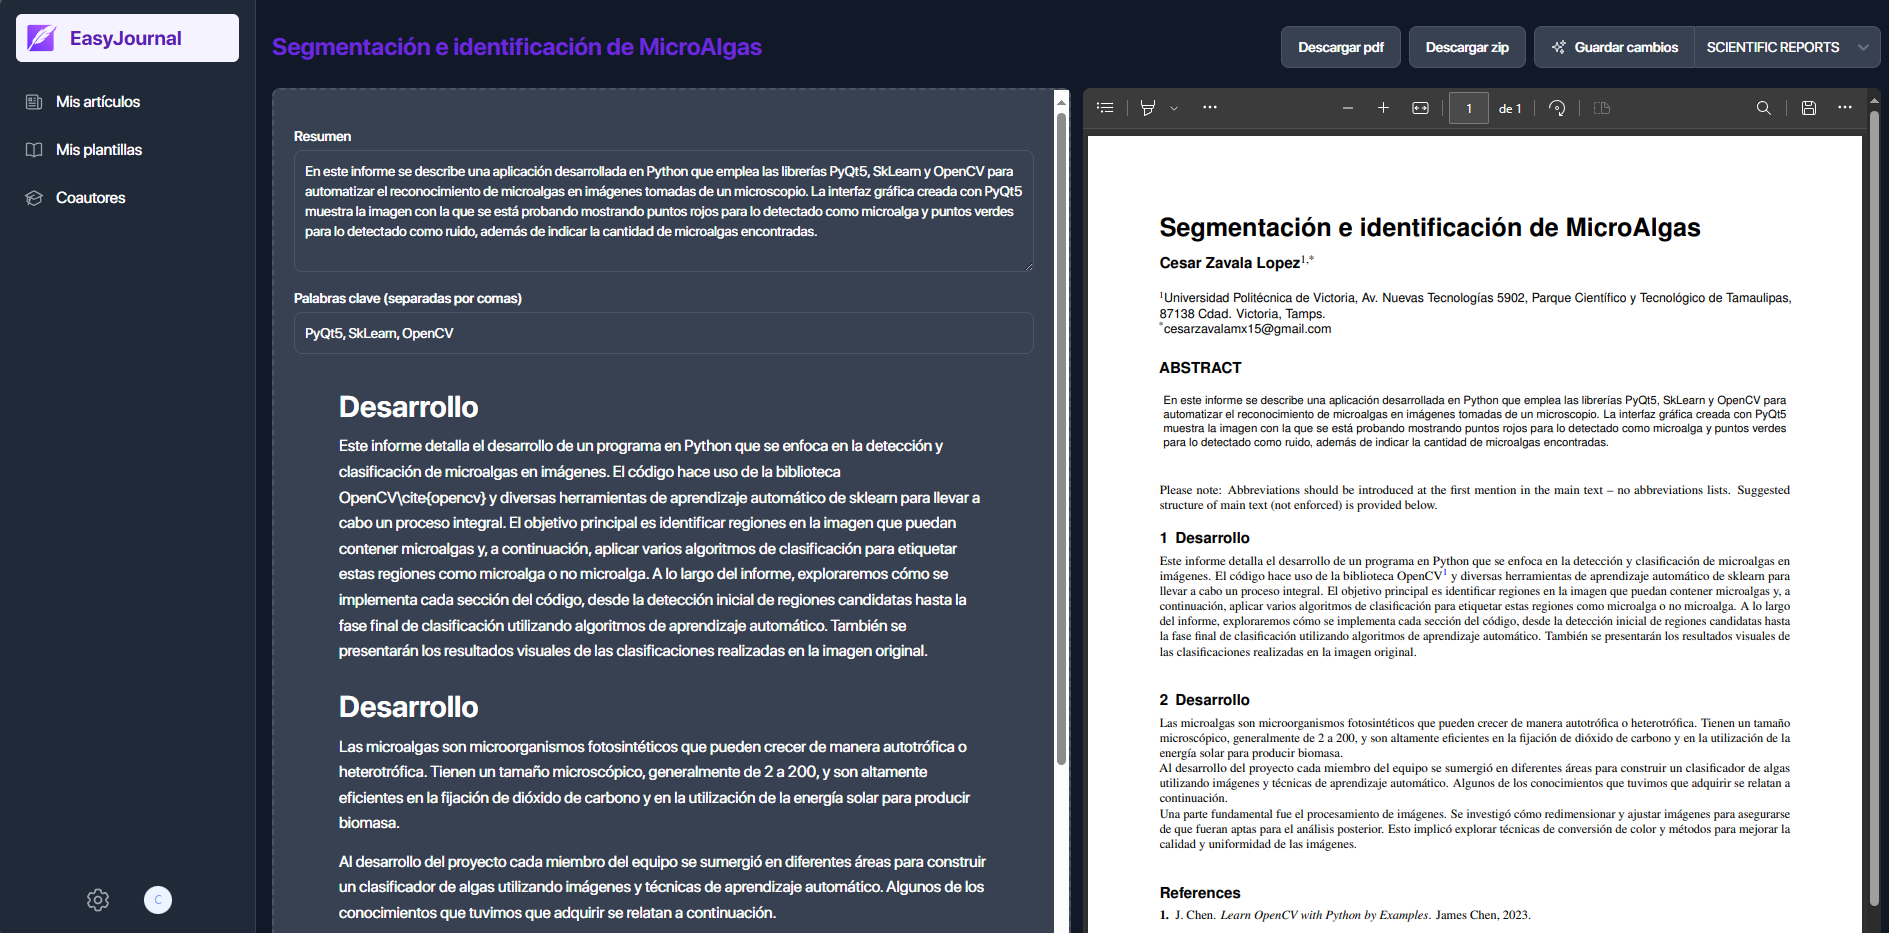
\includegraphics[width=1\textwidth]{IMAGENES/captura-11.png}
    \caption{Página de Edición de Artículo con plantilla Scientific Reports}
    \label{fig:captura-11}
\end{figure}

En la figura \ref{fig:captura-12} se muestra el resultado de la página de edición de artículo compilando la plantilla PeerJ.

\begin{figure}[H]
    \centering
    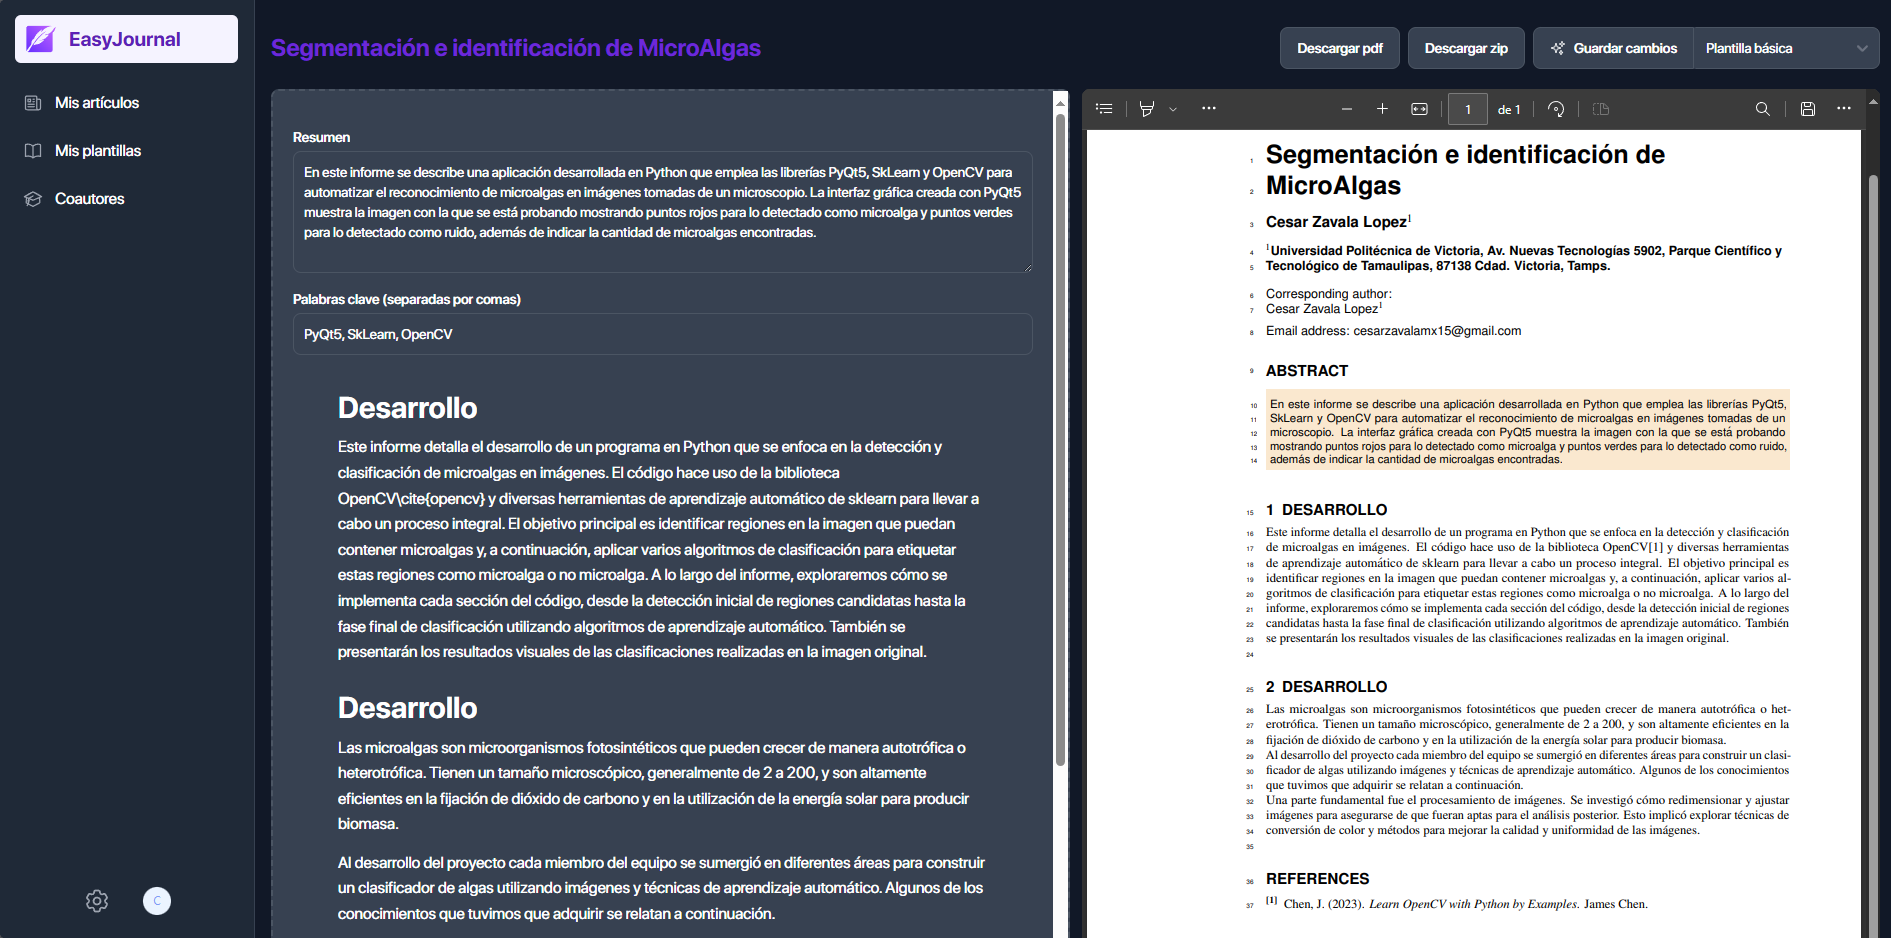
\includegraphics[width=1\textwidth]{IMAGENES/captura-12.png}
    \caption{Página de Edición de Artículo con plantilla PeerJ}
    \label{fig:captura-12}

\end{figure}

En la figura \ref{fig:captura-13} se muestra el resultado de la página de edición de artículo compilando la plantilla IEEE Access.

\begin{figure}[H]
    \centering
    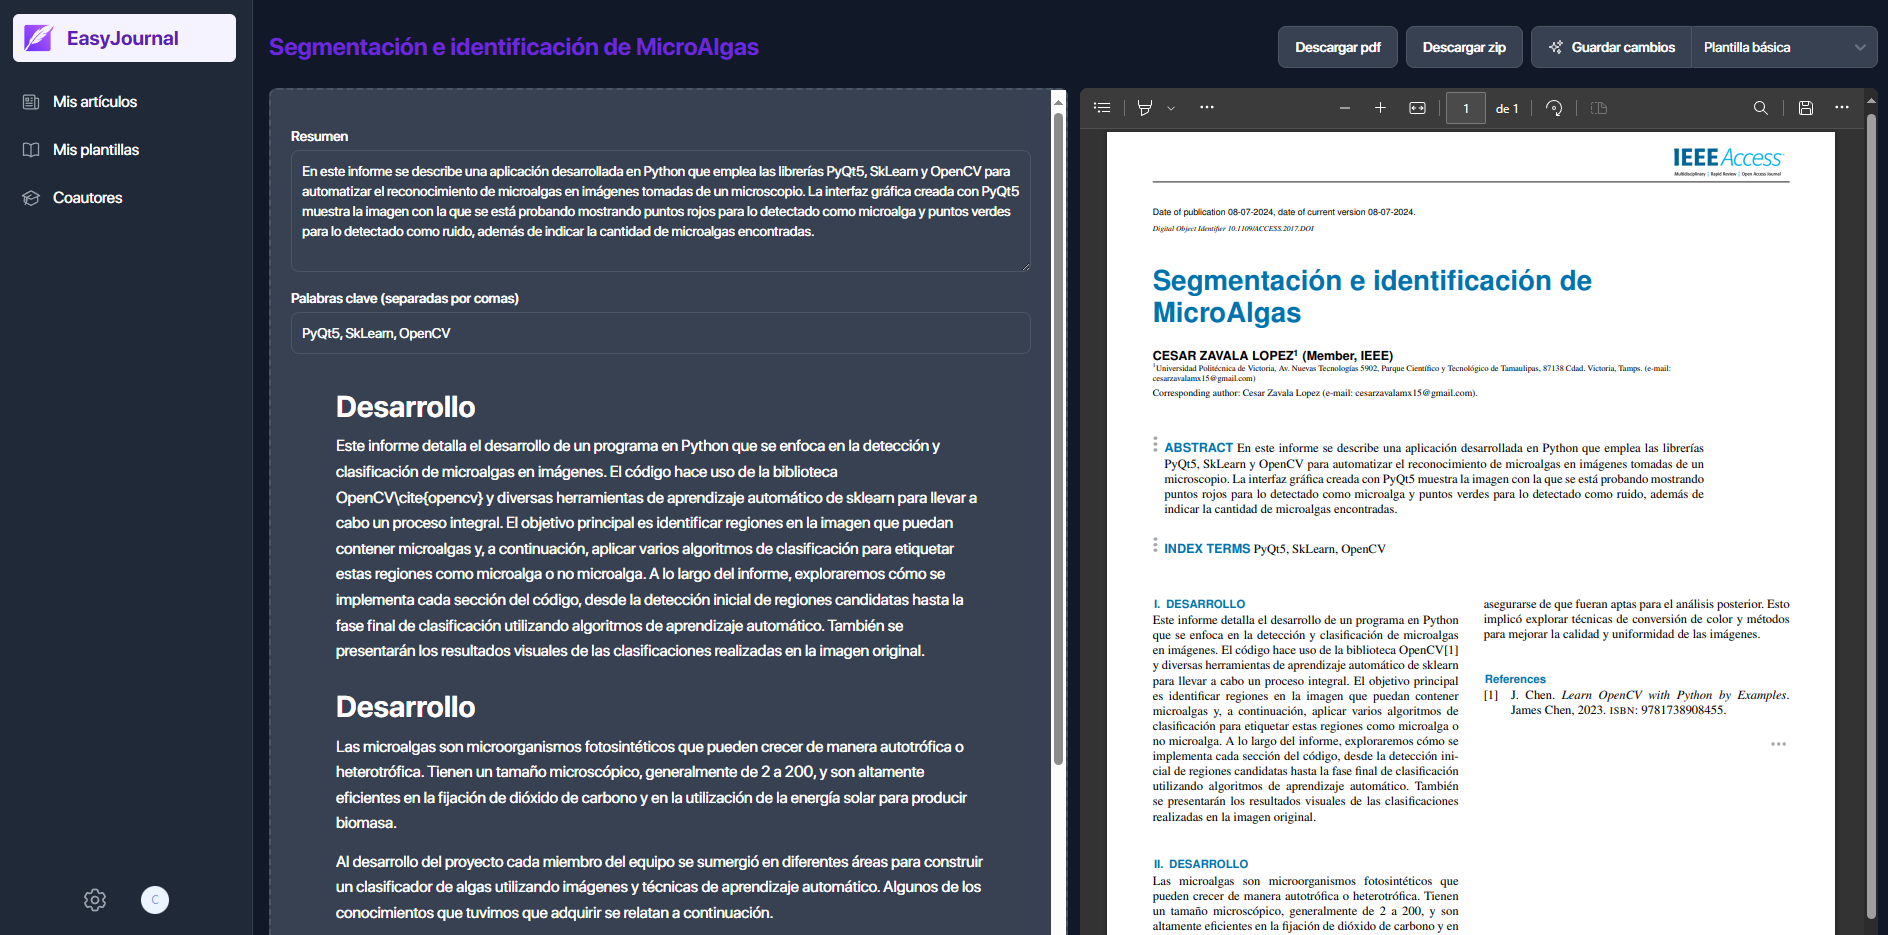
\includegraphics[width=1\textwidth]{IMAGENES/captura-13.png}
    \caption{Página de Edición de Artículo con plantilla IEEE Access}
    \label{fig:captura-13}
\end{figure}

\subsection{Análisis y Discusión de Resultados}
Los logros obtenidos durante el desarrollo del sistema son significativos y demuestran que el sistema cumple con los objetivos establecidos. Se implementaron todas las funcionalidades propuestas y se realizaron pruebas para garantizar el funcionamiento del sistema. Los resultados obtenidos muestran que todas las funcionalidades implementadas funcionan correctamente y que los usuarios pueden interactuar con el sistema de manera eficiente y sin problemas.

A continuación se presentan los logros principales del proyecto:

\begin{itemize}
    \item Se logró integrar Jetstream en el backend del sistema, lo que permitió establecer una base sólida de gestión de usuarios y facilitó el desarrollo de la aplicación.
    \item Se implementó un sistema de gestión de plantillas LaTeX que permite a los usuarios subir plantillas en formato .zip, previsualizarlas y compilarlas en archivos PDF.
    \item Se implementó un sistema de gestión de artículos que permite a los usuarios crear, editar y compilar artículos en plantillas LaTeX.
    \item Se implementó un sistema de gestión de coautores que permite a los usuarios agregar, editar y eliminar coautores de un artículo.
    \item Se implementó un sistema de gestión de archivos que protege los archivos de acceso no autorizado y garantiza la seguridad de los datos.
    \item Se implementó un sistema de validación de plantillas que verifica la estructura y los archivos de la plantilla antes de compilarla.
    \item Se implementó un sistema de seguridad que protege el sistema contra ataques de inyección SQL, XSS, CSRF, fuerza bruta y exposición de datos sensibles.
\end{itemize}   

El impacto del sistema se espera que sea significativo, ya que proporciona una solución innovadora y eficiente para la creación y edición de artículos científicos en formato LaTeX. La implementación de esta herramienta permite a los usuarios generar documentos de alta calidad de manera rápida y sencilla, lo que facilita la colaboración y la comunicación en el ámbito académico y científico. 

